This study employs a qualitative approach where we observe both novices and
experts who's mother tongue is Tamil solving a variety of prompting exercises.
In Section~\ref{sec:eipl-activities} we cover the the variety of prompting
activities we use as the means of exploring how users prompt in Tamil. In
Section~\ref{sec:data-collection-analysis} we cover the data collection and
analysis we employ in investigating our research questions.

\section{Explain in Plain Language Activities}\label{sec:eipl-activities}

\begin{figure}
    \centering
    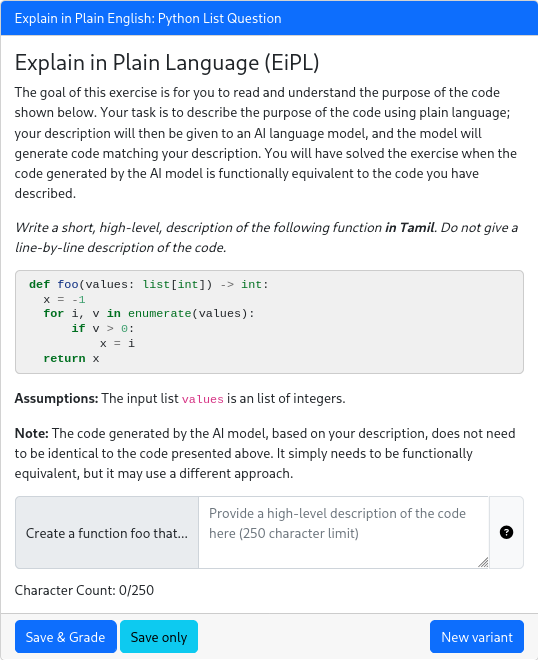
\includegraphics[width=0.95\linewidth]{imgs/eipl-tamil.png}
    \caption{An ``Explain in Plain Language'' Activity}
    \label{fig:enter-label}
\end{figure}

To explore how novices and experts alike approach prompting large language
models when articulating computational tasks we employ ``Explain in Plain
Language'' activities. This activity is derived from the ``Explain in Plain
English'' task which is commonly used in introductory programming courses to
evaluate the ability to comprehend code and articulate its purpose in natural
language. 

\section{Data Collection}\label{sec:data-collection-analysis}

\section{Analysis}\label{sec:analysis}